The logarithm terms are integrated in much the same way they were in the first mandatory assignment.
The boundary element method assumes the potential is constant, set to the value of the midpoint between nodes.
Integration of the logarithm terms in the \textsc{Green} function is outlined in the lecture notes from January 28\textsuperscript{th}.
The gradient of the other terms are given to be
\[
    \deex\green = \kappa \big( \Im{(f_1(\ezh))} + i \Im{(f_2(\ezh))} \big),
\]\[
    \deey\green = \kappa \big( \Re{(f_1(\ezh))} + i\Re{(f_2(\ezh))} \big),
\]
and are treated with a midtpoint rule, setting the complex variable
\[
    \ezh = \kappa\big(\che_m  + \che_n - i (\zhe_m  - \zhe_n) \big).
\]
The boundary we discretize with a \textsc{Chebyshov} distribution in two coordinates $\xtt_\mathtt{p}$ and $\xtt_\mathtt{m}$.
Constructing a partition of the interval whose midpoints forms \textsc{Chebyshov} distribution seems to be more effort than it is worth, so we concede that \textsc{Chebyshov} distributions in $\xtt_{\mathtt{p}}$ and $\xtt_{\mathtt{m}}$ suffice to get accurate enough results near the corners of the box.
\begin{Figure}
    \centering
    \captionsetup{type = figure}
    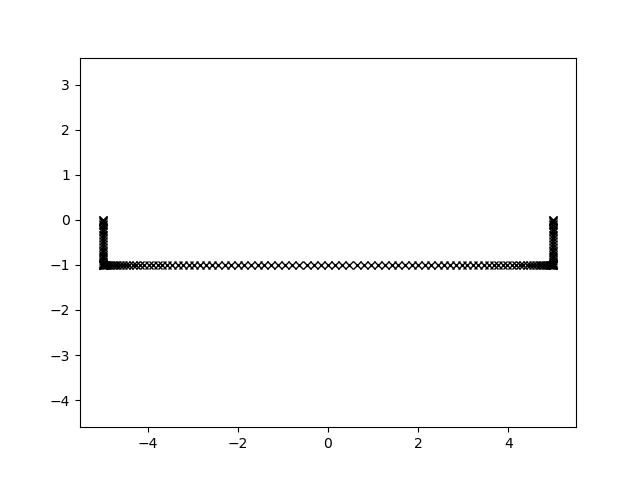
\includegraphics[width = \textwidth]{box_L10.png}
    \caption{Rectangle with $\sfrac{L}{D} = 10$, $\textit{\texttt{N}}_x = 100$, $\textit{\texttt{N}}_y = 25$.}
\end{Figure}
\noindent We may test the numerical scheme by checking that the left-hand side equals the right-hand side of the matrix equation for the real and imaginary parts, using a known function.
We consider
\[
    \phi_0 = \frac{i \gravity e^{\kappa(y-ix)}}{\omega}, \qquad \partial_{\nhat}\phi_0 = \kappa ( \hat{n}_y - i \hat{n}_x ) \phi_0.
\]
We have that
\[
    \pi \phi_0 + \int_{S_{\mathrm{B}}} \phi_0 \partial_{\nhat} \green \,\dee S = \int_{S_{\mathrm{B}}} \green \partial_{\nhat} \phi_0 \,\dee S,
\]
meaning we may benchmark the implementation of the integral equation by comparison.
Plotting the left-hand side against the right-hand side,
\begin{Figure}
    \centering
    \captionsetup{type = figure}
    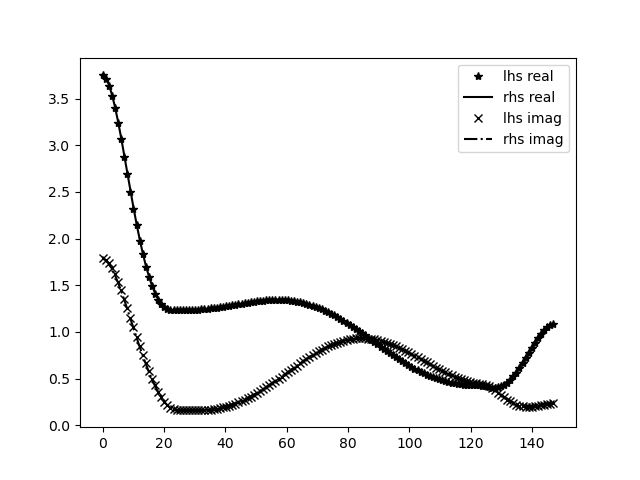
\includegraphics[width = \textwidth]{phi0_L2_D1_kD1point2.png}
    \caption{Left-hand and right-hand side of integral equation with $\phi_0$. Rectangle $\sfrac{L}{D} = 2$.}
\end{Figure}
\noindent We see that the implementation seems to work, so we may solve for the heave potential.
\begin{Figure}
    \centering
    \captionsetup{type = figure}
    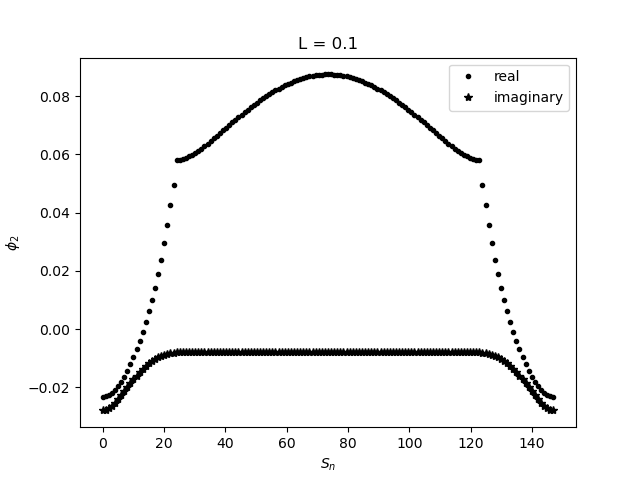
\includegraphics[width = \textwidth]{heave_Lp1_D1_kD1p2.png}
    \caption{Heave potential for $\sfrac{L}{D} = 0.1$, and $\kappa D = 1.2$.}
\end{Figure}
\begin{Figure}
    \centering
    \captionsetup{type = figure}
    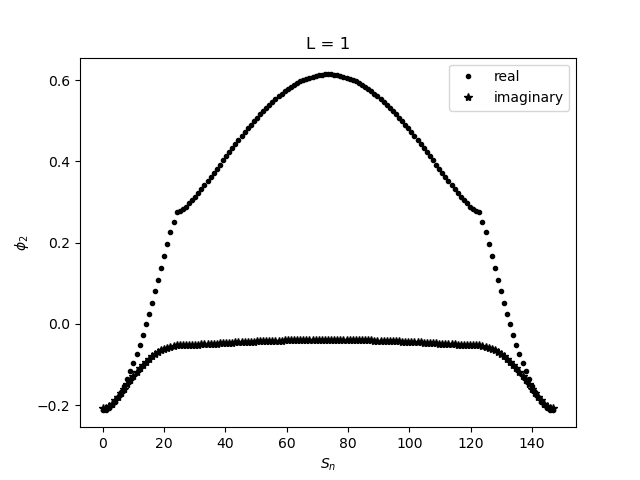
\includegraphics[width = \textwidth]{heave_L1_D1_kD1p2.png}
    \caption{Heave potential for $\sfrac{L}{D} = 1$, and $\kappa D = 1.2$.}
\end{Figure}
\begin{Figure}
    \centering
    \captionsetup{type = figure}
    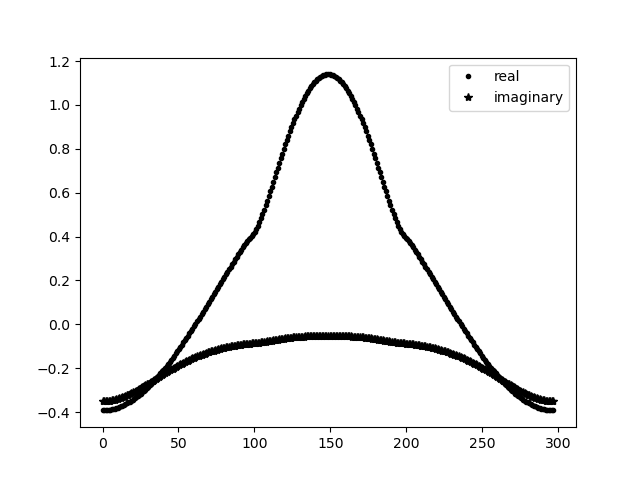
\includegraphics[width = \textwidth]{heave_L2_D1_kD1p2.png}
    \caption{Heave potential for $\sfrac{L}{D} = 2$, and $\kappa D = 1.2$.}
\end{Figure}
\begin{Figure}
    \centering
    \captionsetup{type = figure}
    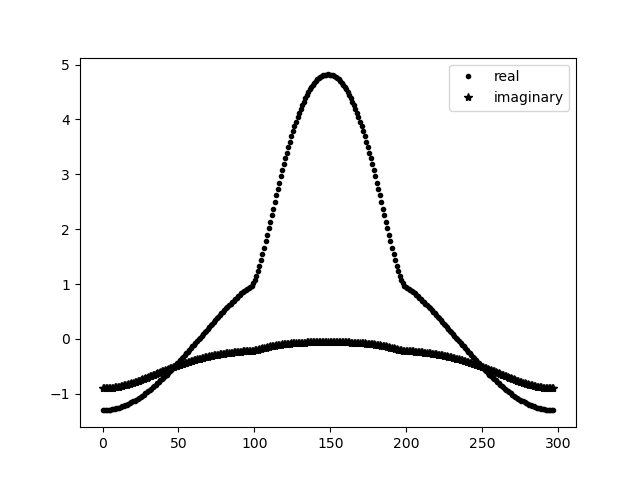
\includegraphics[width = \textwidth]{heave_L10_D1_kD1p2.png}
    \caption{Heave potential for $\sfrac{L}{D} = 10$, and $\kappa D = 1.2$.}
\end{Figure}